\documentclass[10pt]{beamer}

\usetheme{metropolis}

\title{Introduction to Machine Learning}

\begin{document}

\maketitle

\begin{frame}{Concept}

The course is organized as a digital lecture, which should be as self-contained and enable self-study as much as possible:

  \begin{itemize}
    \item
      Slides with lecture videos

    \item
      Interactive tutorials

    \item
       Complemented by a week-long inverted-classroom block course

  \end{itemize}

\end{frame}

\begin{frame}{Concept - Lecture Videos}

  \begin{center}
  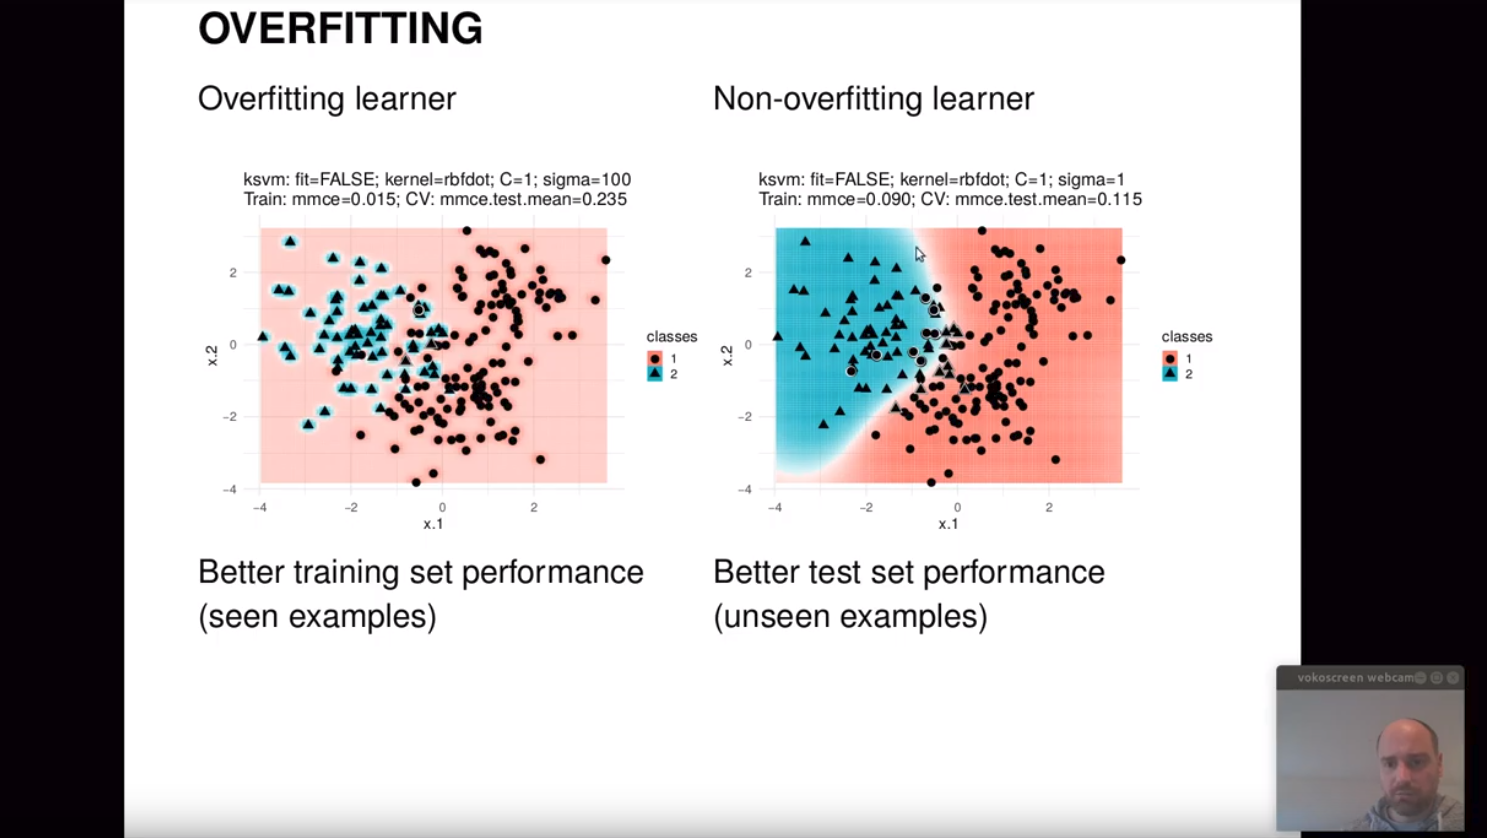
\includegraphics[width=\textwidth]{figures/iml_video.png}
  \end{center}

\end{frame}

\begin{frame}{Concept - Interactive Tutorials (Quiz)}

  \begin{center}
  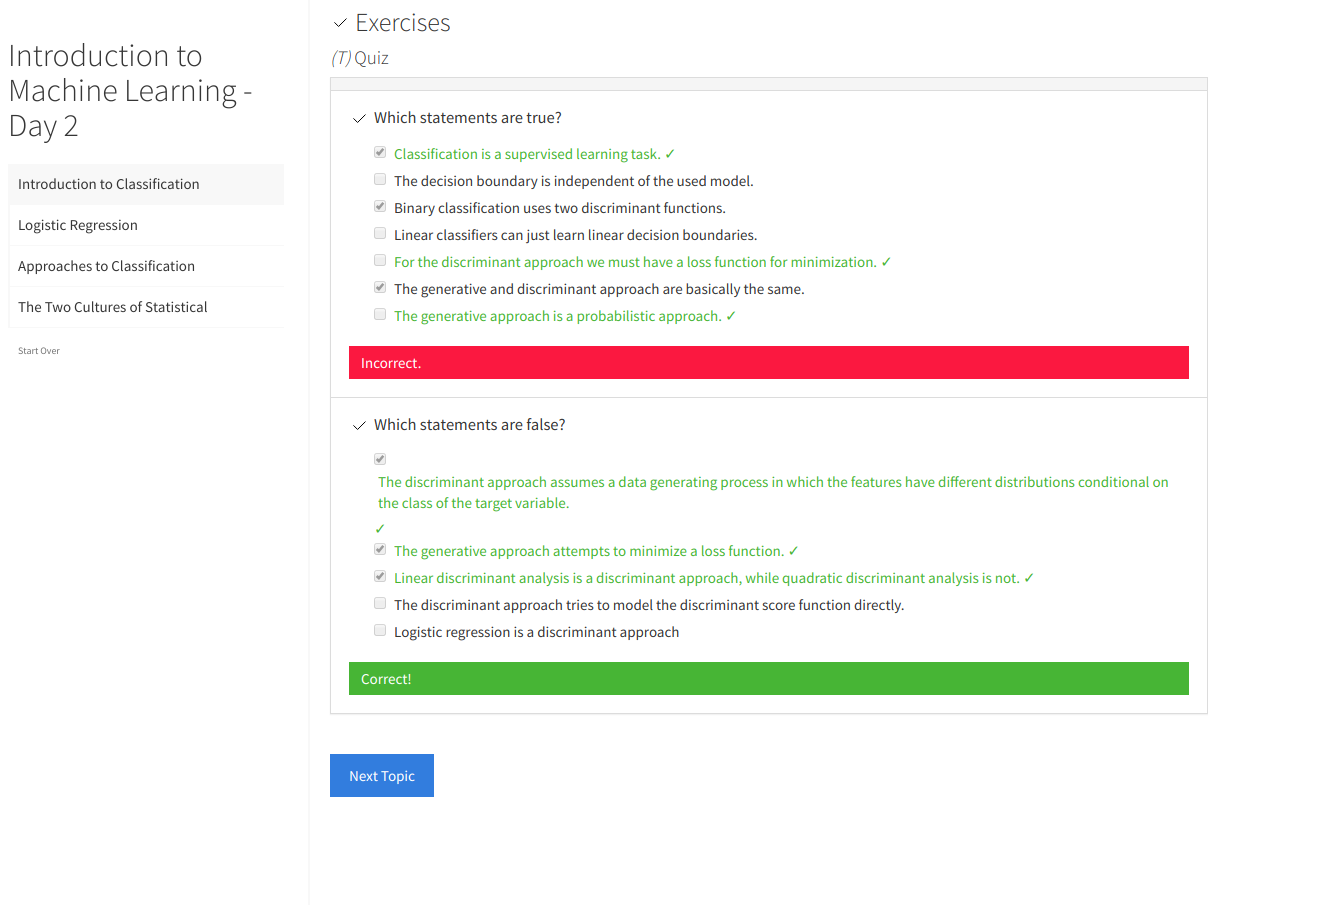
\includegraphics[width=\textwidth]{figures/iml_tut0.png}
  \end{center}

\end{frame}

\begin{frame}{Concept - Interactive Tutorials (Examples)}

  \begin{center}
  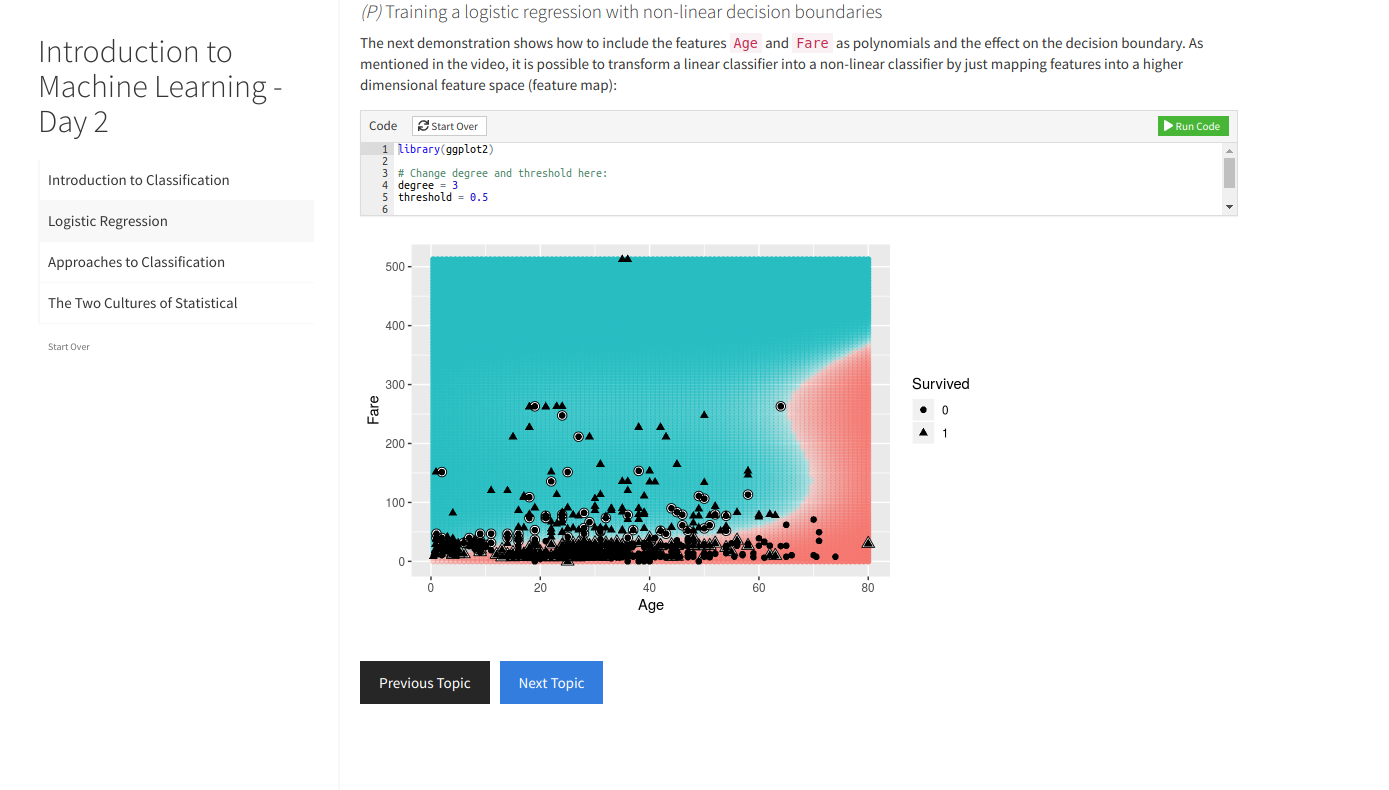
\includegraphics[width=\textwidth]{figures/iml_tut1.png}
  \end{center}

\end{frame}

\begin{frame}

\LARGE{Check it out for yourself:}

\Large{\textbf{\url{compstat-lmu.github.io/lecture_i2ml}}}

\end{frame}


\begin{frame}

Technologies:

\begin{itemize}
\item Videos: very basic free screen-capture programs\\ (\texttt{Kazaam, vokoscreen})
\item Tutorials/Website: (no HTML/CSS skills required)\\
\texttt{Rmarkdown + shiny + learnr + testwhat}
\item Webhosting:
\begin{itemize}
 \item Videos: YouTube (free)
 \item Website: Github (free)
 \item Coding Exercise: \texttt{shinyapps.io} (free for limited traffic)
\end{itemize}
\end{itemize}
\end{frame}

\end{document}
